\section{Trigonometry}

The word ``trigonometry'' comes from the ancient Greek words for ``triangle'' and ``measure'', and it has found its way into just about every possible branch of mathematics and science. You would be putting yourself at a disadvantage not to make sure you are comfortable with at least the basic ideas of trigonometry before continuing to calculus.

You should think about trigonometry in two ways:
\begin{enumerate}
\item pragmatically (it is a useful tool for solving problems, and there are some things you should memorize)
\item abstractly (it is really just a way to talk about similar triangles)
\end{enumerate}

\subsection{Basic Definitions}
The \textbf{unit circle} is the circle with (unit) radius 1, centered at the origin, $(0,0)$. When we draw a radius of the unit circle, it forms an angle $\theta$ with the positive side of the horizontal axis.

\begin{figure}[h!]
\label{sin-cos-coordinates}
\centering
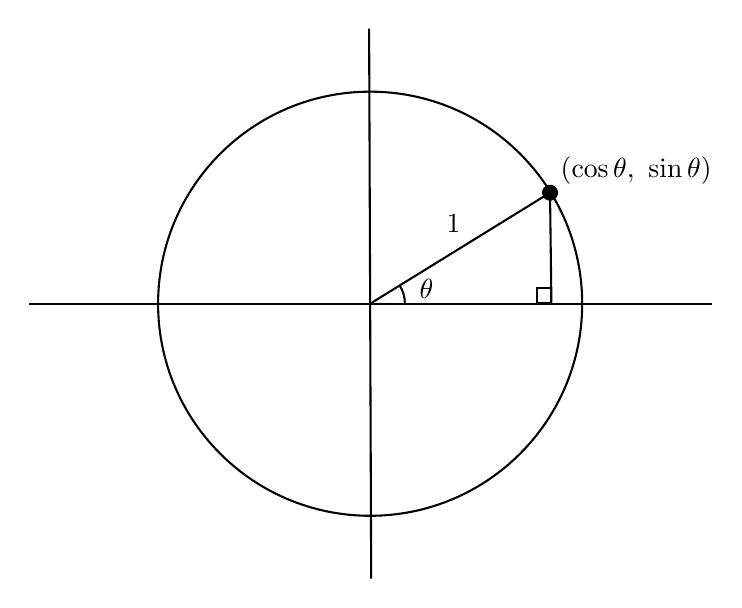
\begin{tikzpicture}[x=0.75pt,y=0.75pt,yscale=-1,xscale=1]
%uncomment if require: \path (0,300); %set diagram left start at 0, and has height of 300

%Shape: Circle [id:dp4792994212957673]
\draw   (247.5,142.5) .. controls (247.5,86.07) and (293.24,40.33) .. (349.67,40.33) .. controls (406.09,40.33) and (451.83,86.07) .. (451.83,142.5) .. controls (451.83,198.93) and (406.09,244.67) .. (349.67,244.67) .. controls (293.24,244.67) and (247.5,198.93) .. (247.5,142.5) -- cycle ;
%Straight Lines [id:da587287090240175]
\draw    (185.17,142.5) -- (514.17,142.5) ;
%Straight Lines [id:da00739473905145327]
\draw    (350.17,275) -- (349.17,10) ;
%Straight Lines [id:da5956961966671213]
\draw    (349.67,142.5) -- (436.33,89) ;
\draw [shift={(436.33,89)}, rotate = 328.31] [color={rgb, 255:red, 0; green, 0; blue, 0 }  ][fill={rgb, 255:red, 0; green, 0; blue, 0 }  ][line width=0.75]      (0, 0) circle [x radius= 3.35, y radius= 3.35]   ;
%Shape: Arc [id:dp01522092049752044]
\draw  [draw opacity=0] (363.84,133.57) .. controls (365.39,136.03) and (366.32,138.92) .. (366.41,142.03) -- (349.67,142.5) -- cycle ; \draw   (363.84,133.57) .. controls (365.39,136.03) and (366.32,138.92) .. (366.41,142.03) ;
%Straight Lines [id:da14866635901795489]
\draw    (436.33,89) -- (437,142) ;
%Shape: Square [id:dp34042868302746565]
\draw   (430,135) -- (437,135) -- (437,142) -- (430,142) -- cycle ;

% Text Node
\draw (372,129) node [anchor=north west][inner sep=0.75pt]    {$\theta $};
% Text Node
\draw (440,70) node [anchor=north west][inner sep=0.75pt]    {$(\cos \theta ,\ \sin \theta )$};
% Text Node
\draw (385,98) node [anchor=north west][inner sep=0.75pt]    {$1$};
\end{tikzpicture}
\caption{$\sin\theta$ and $\cos\theta$ are coordinates}
\end{figure}

This line segment always has length 1, and connects the origin to some point on the circle. We define $\cos\theta$ and $\sin\theta$ to be the $x$ and $y$ coordinates of this point. In other words, $\cos\theta$ is defined to be the (signed) length of the horizontal leg of the right triangle and similarly, $\sin\theta$ is defined to be the (signed) length of the vertical leg.

We measure angles in either degrees or radians. The angle $\theta$ can be any real number, but there are $2\pi$ radians (or 360\degree) in one full revolution. Imagine the angle $\theta$ changing, making the radius sweep around the circle like a SONAR on a submarine. The hypotenuse of the triangle stays constantly at 1, but the side lengths fluctuate between 1 and 0. \mar{Draw a picture: where on the unit circle is $\cos\theta$ positive and where is it negative? How about $\sin\theta$?}

The two functions $\sin$ and $\cos$ are the basic building blocks, but there are four other commonly used trig functions. They are defined as follows:
$$\sec \theta = \frac{1}{\cos\theta}, \quad \quad \csc\theta=\frac{1}{\sin\theta}, \quad \quad \tan\theta=\frac{\sin\theta}{\cos\theta}, \quad \quad \cot\theta=\frac{\cos\theta}{\sin\theta}.$$
These functions also have visual representations on the unit circle.
\begin{figure}[h!]
\centering
\fbox{
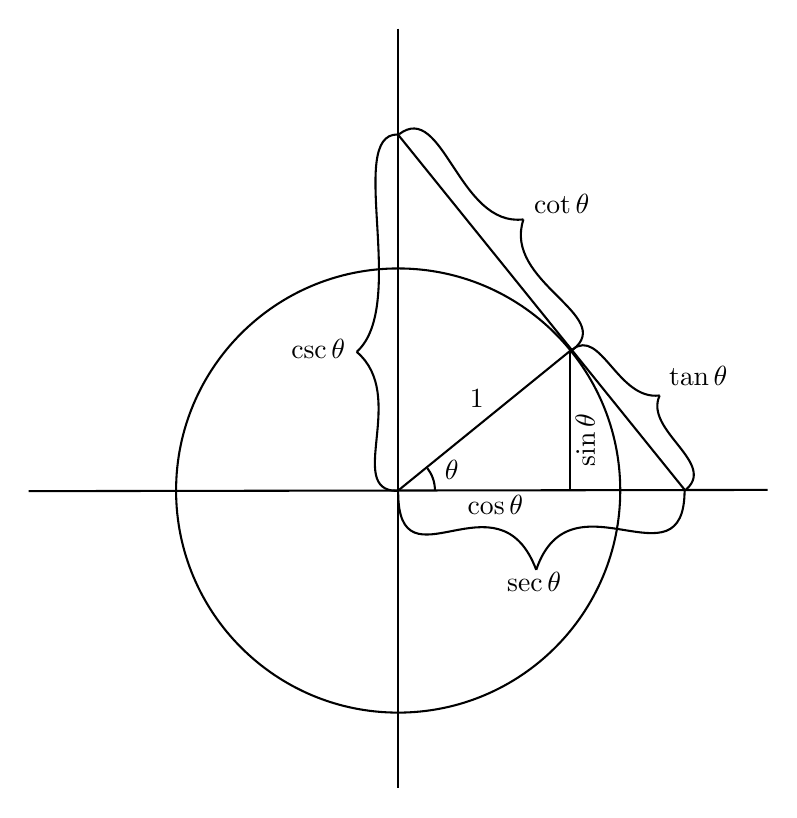
\begin{tikzpicture}[x=0.75pt,y=0.75pt,yscale=-1,xscale=1]
%uncomment if require: \path (0,434); %set diagram left start at 0, and has height of 434

%Shape: Circle [id:dp8118961016990287]
\draw   (214,254.2) .. controls (214,195.11) and (261.91,147.2) .. (321,147.2) .. controls (380.09,147.2) and (428,195.11) .. (428,254.2) .. controls (428,313.29) and (380.09,361.2) .. (321,361.2) .. controls (261.91,361.2) and (214,313.29) .. (214,254.2) -- cycle ;
%Straight Lines [id:da6733376051381585]
\draw    (143,254.5) -- (499,253.9) ;
%Straight Lines [id:da24708595669358502]
\draw    (321,31.7) -- (321,397.7) ;
%Straight Lines [id:da2369525758798794]
\draw    (404,186.8) -- (321,254.2) ;
%Straight Lines [id:da6269364989299404]
\draw    (459,253.8) -- (321,82.8) ;
%Shape: Arc [id:dp8953631465255683]
\draw  [draw opacity=0] (335.11,243.48) .. controls (337.38,246.45) and (338.72,250.17) .. (338.72,254.2) .. controls (338.72,254.26) and (338.72,254.32) .. (338.72,254.39) -- (321,254.2) -- cycle ; \draw   (335.11,243.48) .. controls (337.38,246.45) and (338.72,250.17) .. (338.72,254.2) .. controls (338.72,254.26) and (338.72,254.32) .. (338.72,254.39) ;
%Straight Lines [id:da9446390224381691]
\draw    (404,186.8) -- (404,253.8) ;
%Curve Lines [id:da6889044659660293]
\draw    (321,254.85) .. controls (321,303.53) and (369.22,243.72) .. (387.51,292.4) ;
%Curve Lines [id:da7744827450838345]
\draw    (387.51,292.4) .. controls (404.13,243.72) and (459,302.6) .. (459,253.92) ;
%Curve Lines [id:da7475604962570235]
\draw    (320.73,82.66) .. controls (295.65,82.31) and (326.19,164.99) .. (301,187.4) ;
%Curve Lines [id:da536698622904964]
\draw    (301,187.4) .. controls (325.99,208.44) and (295.33,254.05) .. (320.41,254.4) ;
%Curve Lines [id:da3819978579463683]
\draw    (405.09,186.4) .. controls (426.34,170.03) and (371.15,153.75) .. (381.37,123.57) ;
%Curve Lines [id:da6758383716021474]
\draw    (381.37,123.57) .. controls (350.09,127.39) and (342.7,66.17) .. (321.45,82.55) ;
%Curve Lines [id:da9285330284788131]
\draw    (458.84,254.4) .. controls (476,241.4) and (439,225.4) .. (447,208.4) ;
%Curve Lines [id:da5181742767873634]
\draw    (447,208.4) .. controls (426.87,210.91) and (418.68,175.48) .. (405,186.23) ;

% Text Node
\draw (342,238) node [anchor=north west][inner sep=0.75pt]    {$\theta $};
% Text Node
\draw (372,292) node [anchor=north west][inner sep=0.75pt]   [align=left] {$\displaystyle \sec \theta $};
% Text Node
\draw (268,180) node [anchor=north west][inner sep=0.75pt]   [align=left] {$\displaystyle \csc \theta $};
% Text Node
\draw (385,110) node [anchor=north west][inner sep=0.75pt]   [align=left] {$\displaystyle \cot \theta $};
% Text Node
\draw (450,193) node [anchor=north west][inner sep=0.75pt]   [align=left] {$\displaystyle \tan \theta $};
% Text Node
\draw (353,255) node [anchor=north west][inner sep=0.75pt]   [align=left] {$\displaystyle \cos \theta $};
% Text Node
\draw (405,244) node [anchor=north west][inner sep=0.75pt]  [rotate=-270] [align=left] {$\displaystyle \sin \theta $};
% Text Node
\draw (354,204) node [anchor=north west][inner sep=0.75pt]   [align=left] {$1$};


\end{tikzpicture}
}
\caption{The six common trig functions on the unit circle}
\label{6trig}
\end{figure}


To explore these functions, check out \href{https://www.desmos.com/calculator/fdr54f2jh3}{this graph on Desmos}.


\subsection{Values on the Unit Circle}

There are several angles $\theta$ for which you should be able to compute $\sin\theta$ and $\cos\theta$ (then computing the other four trig functions is easy). Luckily, there is a lot of symmetry involved: it is only necessary to memorize a few numbers and then you can easily fill in the rest.

Below is a diagram of all of the angles whose $\sin$ and $\cos$ you should be familiar with.

\begin{figure}[h!]
\label{the-unit-circle}
\centering
\fbox{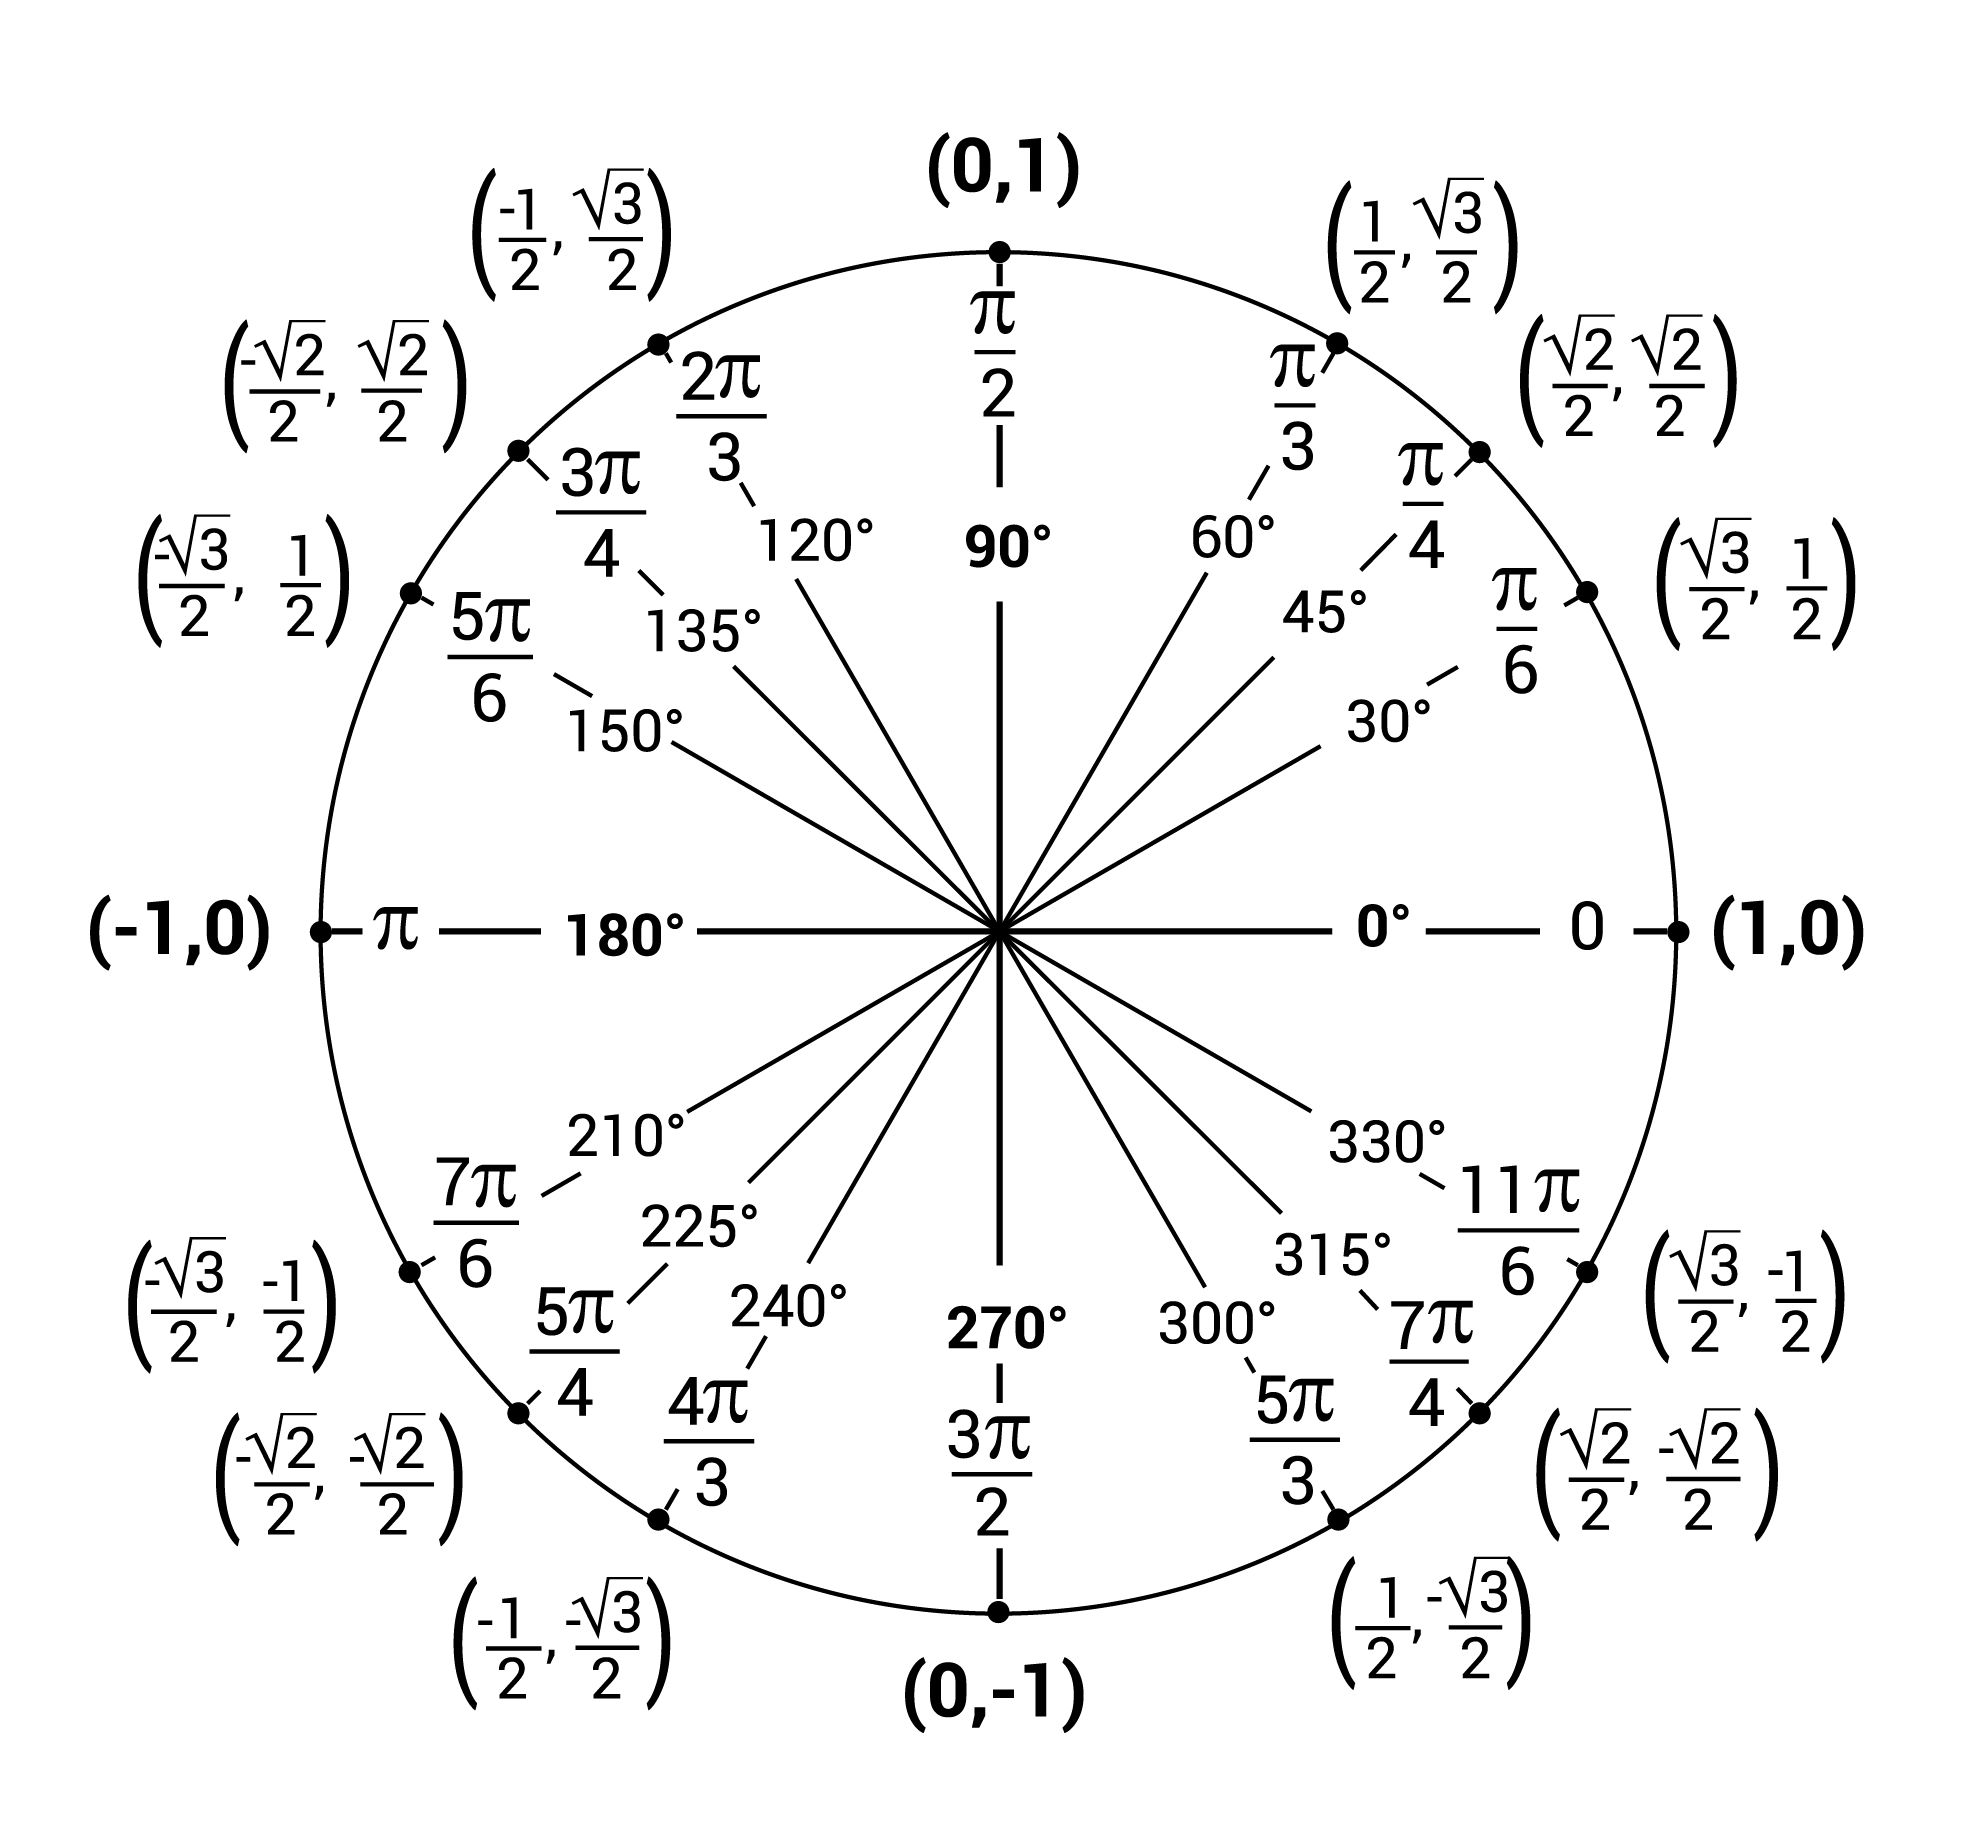
\includegraphics[width=4in]{img/unit-circle.png}}
\caption{The Unit Circle}
\end{figure}


It might seem intimidating, but just focus on the first (upper-right) quadrant and the first five angles there:


\begin{center}
\renewcommand{\arraystretch}{1.3}
\begin{tabular}{@{}lll@{}}
\toprule[0.4mm]
$\theta$ & $\cos\theta$ & $\sin\theta$ \\\midrule
   $0$  & $\sqrt{4}/2$ & $\sqrt{0}/2$ \\
$\pi/6$ & $\sqrt{3}/2$ & $\sqrt{1}/2$ \\
$\pi/4$ & $\sqrt{2}/2$ & $\sqrt{2}/2$ \\
$\pi/3$ & $\sqrt{1}/2$ & $\sqrt{3}/2$ \\
$\pi/2$ & $\sqrt{0}/2$ & $\sqrt{4}/2$ \\\bottomrule[0.4mm]
\end{tabular}
\end{center}

In this table, I wrote the numbers in an ``un-simplified'' way so you can see the pattern: their numerators change by 1 under a square-root, and as one goes up, the other goes down.

You can also see that the values for other angles are the same number, but with a different sign (according to the quadrant they are in), and that the unit circle is symmetric, reflecting over the $x$ and $y$ axis.

\subsection{The Pythagorean and Other Identities}

Remember the Pythagorean Theorem, $a^2 + b^2 = c^2$? Well, since $\sin\theta$ and $\cos\theta$ are the lengths of a right triangle with hypotenuse 1, we have the following \textbf{Pythagorean identity}:
$$\cos^2\theta +\sin^2\theta = 1.$$
\mar{Notation check! Which of the following are the same?
\begin{center}
\begin{tabular}{ c c }
$\sin\theta^2$ & $\sin^2\theta$ \\
$\sin(\theta^2)$ & $\sin(\theta)^2$ \\
$(\sin(\theta))^2$ & $(\sin\theta)^2$ \\
\end{tabular}
\end{center}
}
Dividing this equation by $\sin^2\theta$ or $\cos^2\theta$, we get
$$\cot^2\theta + 1 = \csc^2\theta\quad\quad\text{and}\quad\quad 1+\tan^2\theta = \sec^2\theta.$$

There is some nice symmetry between $\sin\theta$ and $\cos\theta$. The leg opposite the angle is $\theta$ is $\sin\theta$. Since the internal angles of a triangle sum to $\pi$, the other acute angle is $\frac{\pi}{2} - \theta$. \mar{Label the angle $\frac{\pi}{2}-\theta$ on Figure \ref{sin-cos-coordinates}.} Then, the leg opposite $\frac{\pi}{2} - \theta$ has length $\sin\left(\frac{\pi}{2} - \theta\right)$, but is also $\cos\theta$. Therefore,
$$\sin\left(\frac{\pi}{2} - \theta\right) = \cos(\theta).$$
Similarly,
$$\cos\left(\frac{\pi}{2} - \theta\right) = \sin(\theta).$$
Looking at the picture of the unit circle, we can also see that
$$\sin(-\theta) = -\sin(\theta)\quad\text{and}\quad \cos(-\theta)=\cos(\theta).$$

There is one more kind of identity that will be useful for us:
$$\sin(A\pm B)=\sin A \cos B \pm \cos A \sin B,$$
$$\cos(A\pm B)=\cos A \cos B \mp \sin A \sin B.$$

These are called the \textbf{angle sum formulas}, and they are long but if you read them out loud, they make a little song! Try it while clapping on each word:
\begin{center}
``SINE-COSINE-COSINE-SINE. COSINE-COSINE-SINE-SINE.''
\end{center}\mar{No seriously, sing the song. Now do it again.}
Once you remember the order of the functions, you just have to remember that the $A$s and $B$s alternate and that the sign in the second equation flips ($\pm$ becomes $\mp$).

These simplify if $A$ and $B$ are the same angle $\theta$ to what are called the \textbf{double angle formulas}. In this case,
$$\sin(2\theta) = 2\sin\theta\cos\theta$$
and
\begin{align*}
\cos(2\theta) & = \cos^2\theta - \sin^2\theta \\
              & = 1 - 2\sin^2\theta \\
              & = 2\cos^2\theta - 1.
\end{align*}
\mar{Check that these are correct. Hint: use the Pythagorean identity.}

\subsection{Applications}

So, how do we use trigonometry to help solve problems? The main way that trigonometry is useful for you as a calculus student is two-fold. One is as a source of nice function examples to play around with (once we start taking limits and derivatives). The other is as a means to fill in missing information (this is the ``SOH-CAH-TOA'' you might remember).

Let's say you have a right triangle with hypotenuse 8 and one a $30\degree$ angle.


\begin{figure}[h!]
\centering
\tikzset{every picture/.style={line width=0.75pt}} %set default line width to 0.75pt
\fbox{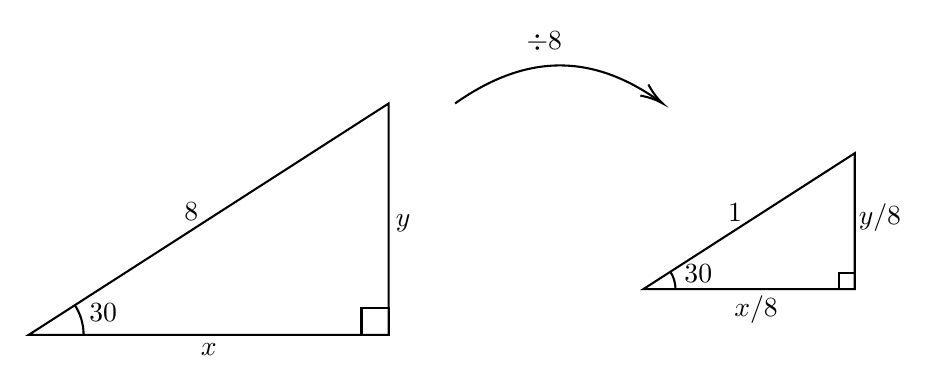
\begin{tikzpicture}[x=0.75pt,y=0.75pt,yscale=-1,xscale=1]
%uncomment if require: \path (0,300); %set diagram left start at 0, and has height of 300

%Shape: Right Triangle [id:dp06753223391248242]
\draw   (236,78) -- (62.56,189.5) -- (236,189.5) -- cycle ;
%Shape: Arc [id:dp8301261755391214]
\draw  [draw opacity=0] (84.77,175.15) .. controls (87.45,179.28) and (89,184.21) .. (89,189.5) -- (62.56,189.5) -- cycle ; \draw   (84.77,175.15) .. controls (87.45,179.28) and (89,184.21) .. (89,189.5) ;
%Shape: Rectangle [id:dp7819843676440785]
\draw   (222.88,176.38) -- (236,176.38) -- (236,189.5) -- (222.88,189.5) -- cycle ;
%Shape: Right Triangle [id:dp36110349096513206]
\draw   (460.53,102) -- (358.65,167.49) -- (460.53,167.49) -- cycle ;
%Shape: Arc [id:dp10101111854625855]
\draw  [draw opacity=0] (371.7,159.07) .. controls (373.27,161.49) and (374.18,164.39) .. (374.18,167.49) -- (358.65,167.49) -- cycle ; \draw   (371.7,159.07) .. controls (373.27,161.49) and (374.18,164.39) .. (374.18,167.49) ;
%Shape: Rectangle [id:dp8285259686836064]
\draw   (452.83,159.79) -- (460.53,159.79) -- (460.53,167.49) -- (452.83,167.49) -- cycle ;
%Curve Lines [id:da345399705785322]
\draw    (268,78) .. controls (303.46,52.98) and (335.04,54.55) .. (366.56,76.96) ;
\draw [shift={(368,78)}, rotate = 216.18] [color={rgb, 255:red, 0; green, 0; blue, 0 }  ][line width=0.75]    (10.93,-3.29) .. controls (6.95,-1.4) and (3.31,-0.3) .. (0,0) .. controls (3.31,0.3) and (6.95,1.4) .. (10.93,3.29)   ;

% Text Node
\draw (90.25,173) node [anchor=north west][inner sep=0.75pt]    {$30\degree $};
% Text Node
\draw (136,124.4) node [anchor=north west][inner sep=0.75pt]    {$8$};
% Text Node
\draw (144,192) node [anchor=north west][inner sep=0.75pt]    {$x$};
% Text Node
\draw (238,130) node [anchor=north west][inner sep=0.75pt]    {$y$};
% Text Node
\draw (377,154) node [anchor=north west][inner sep=0.75pt]    {$30\degree $};
% Text Node
\draw (398,125) node [anchor=north west][inner sep=0.75pt]    {$1$};
% Text Node
\draw (401,169) node [anchor=north west][inner sep=0.75pt]    {$x/8$};
% Text Node
\draw (461,125) node [anchor=north west][inner sep=0.75pt]    {$y/8$};
% Text Node
\draw (301,42) node [anchor=north west][inner sep=0.75pt]    {$\div 8$};


\end{tikzpicture}}
\caption{Similar Triangles}
\end{figure}

If you want to know what the other side lengths are, this is how you can use trigonometry to do it! First, scale the triangle down by the side length that you know (in this case $8$). This doesn't change the angles, so we now have a right triangle with hypotenuse 1. By definition of $\sin$ and $\cos$,
$$\sin 30\degree = \frac{y}{8}\quad\quad\text{and}\quad\quad\cos 30\degree=\frac{x}{8},$$
so we can solve for $x$ and $y$:
$$y = 8\sin 30\degree = 4\quad\quad\text{and}\quad\quad x= 8\cos 30\degree= 4\sqrt{3}.$$
The mnemonic device ``SOH-CAH-TOA'' reminds us that \underline{S}in of $30\degree$ is the \underline{O}pposite leg ($y$) over the \underline{H}ypotenuse (8), and \underline{C}os of $30\degree$ is the \underline{A}djacent leg ($x$) over the \underline{H}ypotenuse (8). \mar{What does the ``TOA'' part say? What situation would it help you figure something out about a triangle?}

The identities that we learned about also have many applications, but mostly are in simplifying calculuations. You should keep them in mind so you recognize when they might be helpful in simplifying an expression. Here is a cool example:
\begin{align*}
\sin\left(2\theta\right)\left(\frac{\tan \theta+\cot \theta}{2}\right)
& = 2\sin\theta\cos\theta\left(\frac{\frac{\sin\theta}{\cos\theta}+\frac{\cos\theta}{\sin\theta}}{2}\right)\\
& = \sin\theta\cos\theta\left(\frac{\sin\theta}{\cos\theta}+\frac{\cos\theta}{\sin\theta}\right)\\
& = \sin^2\theta+\cos^2\theta\\
& = 1.
\end{align*}


Trig identities can also be a computationally useful tool: if you need to know the Sine (or Cosine, etc.) of an angle you are not familiar with, write the angle as a sum or difference of angles you know and use the angle sum formulas. For example,
\begin{align*}
\cos(15\degree) & = \cos(45\degree-30\degree) \\
                & = \cos(45\degree)\cos(30\degree)+\sin(45\degree)\sin(30\degree) \\
                & = \frac{\sqrt{2}}{2}\frac{\sqrt{3}}{2} + \frac{\sqrt{2}}{2}\frac{1}{2} \\
                & = \frac{\sqrt{6}+\sqrt{2}}{4}.
\end{align*}
\mar{Can you compute $\tan(75\degree)$?}

\subsection{There's Always More Trigonometry...}

Trigonometry dates back to the 3rd century BCE and needless to say it has changed a bit over the years. We've only covered the basics and focused on the trigonometry involving right triangles. There is always more trigonometry to learn: more trigonometric functions and MANY more relations among them! I won't pester you with many more right now, but they might come up in the future, so just be aware.

The two very common laws of trigonometry that involve non-right triangles are the Law of Sines and the Law of Cosines. I will state them here (for culture).

\begin{figure}[!h]
\centering
\label{circumscribed-triangle}
\tikzset{every picture/.style={line width=0.75pt}} %set default line width to 0.75pt

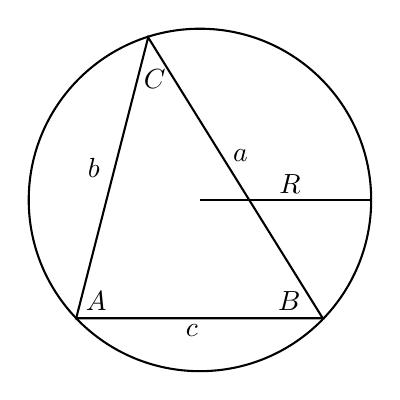
\begin{tikzpicture}[x=0.75pt,y=0.75pt,yscale=-1,xscale=1]
%uncomment if require: \path (0,476); %set diagram left start at 0, and has height of 476

%Shape: Circle [id:dp3720781821561441]
\draw   (155,137.5) .. controls (155,91.94) and (191.94,55) .. (237.5,55) .. controls (283.06,55) and (320,91.94) .. (320,137.5) .. controls (320,183.06) and (283.06,220) .. (237.5,220) .. controls (191.94,220) and (155,183.06) .. (155,137.5) -- cycle ;
%Shape: Triangle [id:dp2721155840135763]
\draw   (212.55,59.19) -- (296.67,194.5) -- (177.87,194.5) -- cycle ;
%Straight Lines [id:da18934326053160722]
\draw    (237.5,137.5) -- (320,137.5) ;

% Text Node
\draw (252,111.82) node [anchor=north west][inner sep=0.75pt]    {$a$};
% Text Node
\draw (181,180) node [anchor=north west][inner sep=0.75pt] {$A$};
% Text Node
\draw (273.69,180) node [anchor=north west][inner sep=0.75pt] {$B$};
% Text Node
\draw (209,73) node [anchor=north west][inner sep=0.75pt]    {$C$};
% Text Node
\draw (229.18,196) node [anchor=north west][inner sep=0.75pt]    {$c$};
% Text Node
\draw (182,116.07) node [anchor=north west][inner sep=0.75pt]    {$b$};
% Text Node
\draw (274.32,123.82) node [anchor=north west][inner sep=0.75pt]    {$R$};


\end{tikzpicture}
\caption{Circumscribed Triangle}
\end{figure}

Figure \ref{circumscribed-triangle} shows a triangle with internal angles $A$, $B$, and $C$, and respective opposite side lengths $a$, $b$, and $c$. The triangle is \textbf{circumscribed} in a circle, meaning its vertices lie on the circle's boundary. It turns out that the circle has radius
$$R=\frac{abc}{\sqrt{(a+b+c)(a-b+c)(a+b-c)(-a+b+c)}}.$$



\begin{thm}[Law of Sines]
If a triangle has sides and angles as above, then
$$\frac{a}{\sin A}=\frac{b}{\sin B}=\frac{c}{\sin C}=2R=\frac{abc}{2\Delta},$$
where $R$ is the radius of the circumscribed circle and $\Delta$ is the area of the triangle.
\end{thm}

\begin{thm}[Law of Cosines]
If a triangle has sides and angles as above, then
$$a^2+b^2=c^2+2ab\cos C.$$
\end{thm}
\mar{Almost looks familiar, right?}

When you use these formulas, keep in mind that solving for an angle can be tricky: if $\sin\theta=1/2$, then $\theta$ could be $30\degree$, $150\degree$, $390\degree$, etc..

Here is one last (very pretty) theorem:
\begin{thm}[Heron's Formula]
A triangle with side lengths $a$, $b$, and $c$ has area
$$\sqrt{s(s-a)(s-b)(s-c)},$$
where $s=\frac{a+b+c}{2}$.
\end{thm}
\mar{Prove this formula.}


